\documentclass[11pt,oneside,final]{fithesis2}
\usepackage[english]{babel}
\usepackage[utf8]{inputenc}
\usepackage[T1]{fontenc}
\usepackage{graphicx}
\usepackage{sidecap}
\usepackage{listings}
\usepackage{float}
\usepackage{url}
\usepackage[plainpages=false, pdfpagelabels, unicode]{hyperref}
\usepackage{enumitem}
\usepackage{algorithm}
\usepackage{algpseudocode}
\usepackage[english]{varioref}
\usepackage{cite}

\usepackage{color}
\definecolor{gray}{rgb}{0.4,0.4,0.4}
\definecolor{darkblue}{rgb}{0.0,0.0,0.6}
\definecolor{cyan}{rgb}{0.0,0.6,0.6}
\definecolor{lightgray}{rgb}{0.9,0.9,0.9}
\definecolor{black}{rgb}{0,0,0}
\definecolor{darkgray}{rgb}{0.2,0.2,0.2}
\definecolor{almostblack}{rgb}{0.1,0.1,0.1}

\lstset{
  basicstyle=\ttfamily,
  columns=fullflexible,
  showstringspaces=false,
  commentstyle=\color{gray}\upshape,
  breaklines=true,
  breakatwhitespace=false,
  xleftmargin=.15in,
  xrightmargin=.15in,
  tabsize=5,
  framexleftmargin=0.1in,
  framexrightmargin=0.1in
}

\lstdefinelanguage{XML}
{
  morestring=[b]",
  morestring=[s]{>}{<},
  morecomment=[s]{<?}{?>},
  stringstyle=\color{almostblack},
  identifierstyle=\color{black},
  keywordstyle=\color{darkgray},
  morekeywords={xmlns,version,type,cd}
}

\thesistitle{Normative Textual Representation of Mathematical Formulae}
\thesissubtitle{Master's thesis}
\thesisstudent{Maro{\v s} Kucbel}
\thesiswoman{false}
\thesislang{en}
\thesisfaculty{fi}
\thesisyear{2013}
\thesisadvisor{doc. RNDr. Petr Sojka, Ph.D.}

\begin{document}
\sloppy

\hyphenation{Math-ML}
\hyphenation{spe-cial-ized}
\hyphenation{style-sheet}
\hyphenation{sche-ma-ta}
\hyphenation{great-ly}
\hyphenation{mark-up}


\setlist[itemize,1]{leftmargin=10pt,itemindent=10pt}
\setlist[itemize,2]{label=$\bullet$}

\FrontMatter
\ThesisTitlePage

\begin{ThesisDeclaration}
\DeclarationText
\AdvisorName
\end{ThesisDeclaration}

\begin{ThesisThanks}
@todo Thanks!
\end{ThesisThanks}

\begin{ThesisAbstract}
@todo Abstract
\end{ThesisAbstract}

\begin{ThesisKeyWords}
MathML, StAX  @todo more
\end{ThesisKeyWords}

\MainMatter
\tableofcontents

\chapter{Introduction}
Mathematics expresses most of its ideas with the help of formulae. To understand a~mathematical formula, the reader needs to interpret not only individual symbols but the layout of the formula as well. In this, mathematical equations resemble two dimensional graphics more than ordinary plain text. However, working with images of mathematical formulae is rather impractical. Editing, copying, and manipulation are very difficult, if not impossible. In spite of these shortcomings of images, they were the main method of including mathematical content in Web pages. For display purposes, it is enough. For further processing of mathematical equations, it is not enough. 

A new format was introduced~- MathML. MathML stems from XML and is, therefore, difficult to read by humans. On the other hand, it is suitable for machine processing. Web browsers are capable of displaying MathML for human readers, and specialized software uses MathML as a~format for data storage and exchange. 

Now we can easily include mathematical content in Web pages or any other XML document, and display it to the user. But what happens if the user is dyslexic, blind, or otherwise visually impaired? There are multiple solutions: conversion to Braille, screen readers, or text-to-speech software. However, with a~few exclusions, their support of mathematics is very slim or nonexistent. Also, search services usually work with plain text only. It is, therefore, desirable to develop a~system that will convert mathematical content inputted in MathML into plain text format. 

This thesis is a~continuation of my Bachelor thesis, \textit{Generování textu~z MathML}~\cite{Kucbel2011thesis}, where a~system for converting MathML data to plain text is created. The goal if the thesis is to significantly improve the developed system. The thesis first looks at the structure of MathML (Chapter~\ref{chapter:mathml}). It then proceeds to list existing accessibility solutions (Chapter~\ref{chapter:statusquo}). Based on the analysis of the problem (Chapter~\ref{chapter:analysis}) an implementation is created (Chapter~\ref{chapter:implementation}). The final chapter provides a~look at results of running the application on real-life data (Chapter~\ref{chapter:results}).

\chapter{Mathematical Markup Language~- MathML}
\label{chapter:mathml}
World Wide Web pages and their main publishing language, HTML\footnote{HyperText Markup Language}, provide many ways to present desired information to the user. However, presenting mathematics is not so easy and straightforward. There aren't any special tags in the HTML specification for including mathematical content. In most cases mathematical equations are presented in the form of an image. On one hand this approach renders the equation the same way in every web browser, on the other hand there is no way to copy the equation for further use, not to mention editing the equation. 

MathML\footnote{\url{http://www.w3.org/Math/}} was specifically created to circumvent this obstacle. It was designed to be used in web pages along with HTML. It follows that MathML is an application of XML with special set of tags used to capture the content, structure, and even presentation details of mathematical equations. We will take a~closer look at how this is achieved in the following sections. In April 1998 MathML became the recommendation of the W3C working group\footnote{The World Wide Web Consortium (W3C) is the main international standards organization for the World Wide Web} for including mathematics into web pages.

\section{Structure of MathML}
MathML as an application of XML consists of a~tree of nodes. Each node is either empty, has textual value, or has a~list of descendant nodes. To provide additional information, a~node can have an arbitrary amount of attributes (key – value pairs). Each MathML tree has to have a~root node named \texttt{math} that belongs to the MathML namespace. Also, it is important not to forget to include XML declaration and MathML doctype declaration. 

MathML comes with two distinct sets of tags. For the visual form of equations there are Presentation MathML tags, while Content MathML tags focus on the semantics and meaning of formulas. Presentation tags are being used primarily by web browsers to display mathematical expressions to the users, Content tags are important for further processing of expressions by specialized mathematical programs.

\subsection{Presentation MathML}
The main focus of the Presentation MathML is displaying the equation. For this purpose, there are around thirty elements~- all starting with the prefix “m”. Elements are divided into two classes, first of which is called tokens. It consist of elements that represent individual content and do not contain other nested elements. These include: 
\begin{itemize}
\item \texttt{<mi>x</mi>}~- identifiers,
\item \texttt{<mn>2</mn>}~- numbers,
\item \texttt{<mo>+</mo>}~- operators, fences, separators,
\item \texttt{<mtext>}free text\texttt{</mtext>}~- text.
\end{itemize}
The content of the token can of course be expressed in more than one character (\texttt{<mo>sin</mo>}) or with an XML and HTML character entities. For example, \texttt{\&\#62;} and \texttt{\&gt;} have the same meaning as \texttt{>}~- greater than. It is completely up to the users which notation they will choose.

Even though nesting other elements in tokens is not allowed, there are exceptions. For example, HTML5 allows almost any HTML inline tag inside the \texttt{mtext} element. So \texttt{<mtext><b>free</b> text</mtext>} would be rendered with the bold word free.
The other class of elements is layout schemata. This collection of elements is further divided into following groups:
\begin{itemize}
\item General Layout:
	\begin{itemize}
	\item \texttt{<mrow>}~- general horizontal grouping,
	\item \texttt{<mfrac>}~- fractions and binomial numbers,
	\item \texttt{<msqrt>}, \texttt{<mroot>}~- radicals;
	\end{itemize}
\item Script and Limit~- superscripts, subscripts, 
\item Tabular Math~- tables and matrices,
\item Elementary Math~- notation for lower grades mathematics.
\end{itemize}
We can think of the layout schemata as a~form of expression constructors, that specify the way in which sub-expression are constructed into larger expressions, starting with tokens and ending with the \texttt{math} element. Therefore, elements belonging to layout schemata class do not contain any characters, only other nested elements (layout schemata or tokens). 

\begin{figure}[!ht]
\lstset{language=XML,frame=lines}
\begin{lstlisting}
<math>
	<mrow>
		<mi>e</mi>
		<mo>=</mo>
		<mi>m</mi>
		<mo>*</mo>
		<msup>
			<mi>c</mi>
			<mn>2</mn>
		</msup>
	</mrow>
</math>
\end{lstlisting}
\caption{Expression $e=m \cdot c^2$ in Presentation MathML}
\label{fig:presentationmathml}
\end{figure}

Presentation MathML also provides over fifty attributes for fine tuning of expressions, like setting colors, dimensions, alignments, and many others.

\subsection{Content MathML}
Mathematical notation, rigorous as it is, is still not standardized around the world, and there are many different ways of writing mathematical expressions based on cultural customs. Even simple multiplication operation can be written as $x*y$, $xy$, $x\ times\ y$, $x \times y$. In many situations there's no need to actually render the expression; only the underlying meaning is important. For this reason, the Content MathML provides a~framework and a~markup language that capture the semantics of mathematical expressions.

The structure of the Content MathML tree is based on a~very simple principle – applying an operator to sub-expressions. For example, the quotient $x/y$ can be thought of as applying the division operator to two arguments~- $x$ and $y$. It follows that the cornerstone of the Content MathML is the function application element \texttt{<apply>}.  The first child of the \texttt{<apply>} element signifies the operator, which can be an \texttt{<apply>} element again, and the rest of the \texttt{<apply>} element's direct descendants are arguments to which the operator is applied. Token elements \texttt{<ci>} and \texttt{<cn>} are available to represent numbers and variables respectively. 

The Content MathML provides two ways of defining the operator. The first one is a~set of more than 100 elements each corresponding to some mathematical operator. For example, for the addition operator there is \texttt{<plus>}, for logical xor \texttt{<xor>}, and so on. Then there is the second way~- the element \texttt{<csymbol>}. This element contains a~textual representation of the operator that is bound to a~definition in a~content dictionary referenced by either the attribute \texttt{cd} or \texttt{definitionURL}. External content dictionaries are important for communication between agents, and there exist several public repositories of mathematical definitions. Most notable is the OpenMath Society repository.

\begin{figure}[!ht]
\lstset{language=XML,frame=lines}
\begin{lstlisting}
<math>
	<apply>
		<eq/>
		<ci>e</ci>
		<apply>
			<times/>
			<ci>m</ci>
			<apply>
				<power/>
				<ci>c</ci>
				<cn>2</cn>
			</apply>
		</apply>
	</apply>
</math>
\end{lstlisting}
\caption{Expression $e=m \cdot c^2$ in Content MathML}
\end{figure}

In the MathML 3 a~subset of the Content MathML elements is defined~- the Strict Content MathML. This uses only minimal, but sufficient, amount of elements. Most importantly, it only allows the usage of \texttt{<csymbol>} element for defining operators. The Strict Content MathML is designed to be compatible with the OpenMath standard.

\begin{figure}[!ht]
\lstset{language=XML,frame=lines}
\begin{lstlisting}
<math>
	<apply>
		<csymbol cd="dict">equals</csymbol>
		<ci type="real">e</ci>
		<apply>
			<csymbol cd="dict">times</csymbol>
			<ci type="real">m</ci>
			<apply>
				<csymbol cd="dict">power</csymbol>
				<ci type="real">c</ci>
				<cn type="integer">2</cn>
			</apply>
		</apply>
	</apply>
</math>
\end{lstlisting}
\caption{Expression $e=m \cdot c^2$ in Strict Content MathML}
\end{figure}

\section{Creating MathML Markup}
\label{sec:create-mathml}
Creating MathML documents is very simple. All that is needed is a~word processor available on every operating system. However, this approach is prone to errors, be it the wrong letter case or unclosed tags. Since MathML is an XML language, the usage of some sophisticated word processor that supports tags highlighting, code completion, and XML validation will greatly improve the efficiency of creating MathML documents. But the whole process is still very time consuming and impractical. As is the case with most XML documents, even writing simple mathematical expressions takes up a~lot of space and time. Fortunately, there are many dedicated MathML editors that provide some degree of abstraction from the actual MathML markup.

Multiple software products designated for working with mathematical expressions provide an option to output the results of calculations in MathML format. These include a~popular web service Wolfram Alpha, Mathematica, Maple, or Matlab. MathML can also be used as a~data exchange format or an input format for aforementioned programs.

Another way of creating MathML documents is a~conversion from different formats. Among scientists, mathematicians particularly, \TeX\ is the format of choice. It then comes as no surprise that there are many sources of mathematical texts written in \TeX. However, not every publication comes with the source files. Often only print-ready PDF files are released~\cite{baker2011towards}. Also many academic writings, especially older ones, are available only in printed form. These have to be scanned using an Optical Character Recognition (OCR) software. 

\subsection{\LaTeX ML}
\label{section:latexml}
The lack of a~suitable tool for converting \LaTeX\ to XML prompted the participants of the Digital Library of Mathematical Functions project to develop their own solution. Main goals of \LaTeX ML~\cite{latexml:miller2013} design contain the aspiration to faithfully emulate \TeX\ behavior, the ease of extensibility, and the preservation of both semantic and presentation aspects of original documents. To this end \LaTeX ML provides two main commands~- \texttt{latexml} and \texttt{latexmlpost}. The \texttt{latexml} command converts the initial \TeX\ document to the XML format based on a~set of \LaTeX ML-bindings files that define the mapping of \TeX\ macros to XML. \texttt{latexmlpost} then processes resulting XML output by converting mathematics
and graphics, cross-referencing, and applying an \texttt{XSLT}\footnote{Extensible Stylesheet Language Transformations \url{http://www.w3.org/TR/xslt}} stylesheet. 

Both commands come with a~multitude of parameters that allow users to customize the whole process, such as loading user-defined bindings or choosing the output format. Based on the requested output format mathematics is converted to graphics (png images for HTML) or Presentation MathML in case of XHTML or HTML5. 

\LaTeX ML is freely available online as an installation package for Linux systems as well as Windows and MacOS. An extensive and detailed manual is available online or as a~PDF document.

\subsection{Tralics}
Tralics~\cite{tralics:grimm2003,dml:Grimm2010} is a~freeware software designed to translate \LaTeX\ sources into XML documents that can be further converted into either PDF or HTML. The generated XML is conforming to the local ad-hoc DTD (a simplification of the TEI) with mathematical formulas conforming to the Presentation MathML 2.0 recommendations.

Similarly to \LaTeX ML, Tralics provides many ways for customization of resulting documents, among them the possibility to change element and attribute names in the XML file. Besides Presentation MathML, mathematical formulae can be translated into \LaTeX -like   elements as well.

Tralics is readily available online in the form of source files or binaries for Linux, Windows, and MacOS operating systems. An extensive documentation regarding customization and usage is also available online. 

\subsection{MaxTract}
MaxTract~\cite{baker2012maxtract} is a~tool that through spacial analysis of symbols and fonts in PDF document reverse-engineers its source files in the form of \LaTeX\ or XHTML + MathML documents. The conversion process requires valid PDF files to work correctly as it needs the information about symbols, font encoding, and width of objects contained in the PDF file. PDF documents created via \LaTeX\ fulfill these requirements. As a~result, MaxTract is able to process most of the scientific and mathematical material.


\subsection{INFTY Reader}
INFTY~\cite{suzuki2003infty} is an Optical Character Recognition (OCR) software especially created for mathematical documents. INFTY reads scanned pages (images) and yields their character recognition results in multiple formats, including \LaTeX\ and MathML. It does so in four steps: layout analysis, character recognition, structure analysis of mathematical expressions, and manual error correction (optional). 

The most important phase~- character recognition~- is responsible for distinguishing mathematical expressions and running a~character recognition engine originally developed for mathematical symbols together with non-specialized commercial OCR engine. 

INFTY Reader is available free of charge for limited amount of time, then it is necessary to purchase a~license key.

\subsection{\TeX 4ht}
\TeX 4ht~\cite{tex4ht:gurari2004} is a~system for producing structured output in a~markup language from sources written in the \TeX -based family of languages. It is highly extensible and configurable; most common configurations include the conversion from \LaTeX\ to HTML with MathML, Braille, or DocBook targets.

The conversion is invoked by running the \texttt{htlatex} command. To the user the process seems similar to producing standard DVI or PDF outputs. \TeX 4ht uses hooks within \LaTeX\ constructs and associates configurations to them. By modifying default configuration files, the user can change the resulting HTML document to his liking. \TeX 4ht comes with the support of Cascading style sheets\footnote{\url{http://www.w3schools.com/css/}}, which provides further possibilities of customizing the output files. 

\section{Canonicalization of MathML}
\label{section:canonicalization}
With a~wide variety of options for creating MathML documents, it is necessary to modify and unify input documents in such a~way that will decrease the number of possible ambiguities (especially in the Presentation MathML); in the best case completely eliminating all ambiguities. 

The team standing behind the Universal Maths Conversion library (UMCL)~\cite{umcl:archambault2004towards} proposed a~notion of a~unified structure~- Canonical MathML~\cite{umcl:archambault2006canonical}. Canonical MathML is valid Presentation MathML and recommends a~set of rules that should be followed to make Presentation MathML documents unambiguous. A~correct use of \texttt{msup} (\texttt{msub}) for superscripts (subscripts); parentheses defined in the \texttt{mo} element (\texttt{mfenced} element is not used); or unified way of writing summations, integrals, and products to name a~few. 

UMCL incorporates this notion and provides a~module for converting Presentation MathML markup into Canonical MathML. The canonicalization module employs the use of XSL stylesheets and transformations to create the desired Canonical MathML. However, XSL Transformations tent to be quite slow, and the UMCL canonicalization is rather error-prone, and sometimes even changes the semantics of mathematical formulae, as was shown in M. Jarmar's thesis~\cite[chapter 5]{umcl:jarmar2012conversion}. 

These shortcoming of UMCL prompted a~team at Masaryk University to design and implement their own canonicalization solution~\cite{canonicalization:formaneketal} for use in the (Web)MIaS project~\cite{mias:sojka2011indexing}. Although the implementation of this solution is still under development, the core functionality is already working, and provides better results than UMCL (from the point of performance as well as the structure of converted documents). 

\chapter{Status Quo of Current Tools}
\label{chapter:statusquo}
Making mathematical content available to visually impaired users or those with dyslexia has been a~focus of many projects and researches over the last two decades. As a~result several products (commercial or open source) have been developed that help the users with working with mathematical formulae. By providing text-to-speech solutions, easy to use and comfortable editors, or support for browsing and searching documents that contain mathematical equations.

In this chapter we will present some solutions that are unique in this field, and had impact on another similar products~- either by the theoretical research that fuels such solutions or by general aspects that make them stand out. 

\section{DAISY}
DAISY\footnote{\url{http://www.daisy.org/daisy-standard}} (Digital Accessible Information System) is a~technical standard for digital audio books, periodicals, and computerized text. It is specifically intended for people that have problems reading a~printed text including blindness, dyslexia, or impaired vision. DAISY is based on combination of XML and MP3, and has various functions that traditional audio books do not provide. These include: line by line navigation, searching in the text, adding bookmarks, or adjusting the speed of the speech. It also provides support for embedded content, such as images, graphics, and MathML. 

DAISY books (books conforming to the DAISY standard) can be listened to on designated DAISY readers, computers with installed DAISY software, mobile phones, or MP3 players. There are many implementation of software players~- commercial, free, or even open source. They range from standalone applications to addons for internet browsers (especially Mozilla Firefox). Some software players are capable of displaying HTML pages with embedded MathML markup, and subsequently read the mathematical expressions (this functionality was tested on a~commercial product Dolphin EasyReader that supports Czech language as well).   

\section{MathPlayer}
\label{mathml:mathplayer}
MathPlayer is an application developed by Design Science\footnote{\url{http://www.dessci.com/en/products/mathplayer/}} that enables users of Microsoft Internet Explorer web browser to display mathematical equations written in MathML markup. It uses Microsoft's internal HTML engine (MSHTML) on which Internet Explorer is based. Also, for any application that makes use of MSHTML to display formatted content MathPlayer is able to display MathML content. This may include email clients, alternative browsers, or RSS readers. 

Besides displaying MathML in the browser, MathPlayer comes equipped with a~wide range of MathML-related functions. It enables equations to be copied to the clipboard as MathML markup and pasted to any MathML-aware software~- be it simple text editor or more sophisticated application. Drag-and-drop functionality is also supported. Another important feature of the MathPlayer is the ability to speak expressions on the web page.

MathPlayer is shipped as a~free to use software with English localization only but is still a~close source product. The license limits its use to only computers owned by the user and also prohibits translation and reverse engineering of the application.

\section{AsTeR}
AsTeR (Audio System for Technical Readings) is an exceptional piece of software developed by T.V. Raman as a~part of his dissertation at Cornell University~\cite{aster1994}. AsTeR is capable of producing audio renderings of technical documents, even those containing higher mathematical expressions, written in \TeX\ or \LaTeX. However, processing different markup languages does not pose a~problem for AsTeR. All that is required is a~recognizer for given markup language. 

The logical structure of the document is transformed to an internal representation, which is then rendered in audio using a~collection of rendering rules. This enables AsTeR to provide different views of the document. A~user can listen to the whole document or select a~portion of the document for listening. An important feature of AsTeR makes us of the voice intonation to read long and complicated formuale. Such formulae are divided into logical parts (like a~single summation or a~numerator of a~fraction) and read with different intonation than the surrounding part of the expression. 

\section{MathTalk}
MathTalk~\cite{mathtalk:stevens1994mathtalk} is a~commercial text-to-speech software that enables visually impaired people to read algebra notation in a~quick manner. MathTalk was designed and created as a~part of doctoral dissertation of R. D. Stevens~\cite{mathtalk:stevens1996principles} and employs the use of prosody in the synthetic voice to decrease the mental workload of the listener. MathTalk enables the users to browse the document and change the speed of reading, which gives them comfortable control of the reading process.

\section{Lambda}
Lambda~\cite{lambda:schweikhardt2006lambda} (Linear Access to Mathematic for Braille Device and Audio-synthesis) aims at solving the problem of mathematics text management by blind users. It consists of two sections: the Lambda code and the editor.

The Lambda code directly derives from MathML. It is automatically convertible into equivalent MathML and through it into the most popular mathematical formats. The Lambda code was designed to:
\begin{itemize}
\item have explicit meaning with no ambiguities,
\item provide full Braille output of mathematical equations,
\item preserve peculiarities of national Braille,
\item have a~compact linear representation (minimize the movement while reading Braille).
\end{itemize}
The Lambda editor allows to write and manipulate mathematical expressions. It is essentially a~text editor designed to read and write Lambda code. Mathematical elements are grouped into blocks that can be collapsed or expanded for easier reading. Blocks can also be deleted or copied to a~different place in the document. The output of the Lambda editor can be written (displayed) in Braille, spoken by speech synthesis, or both at the same time. The speech synthesis exploits the block structure, which enables it to change the speech speed and insert brakes to better communicate the meaning of the mathematical formula. 

\section{Web Browser Support}
Strictly speaking, web browsers by themselves are not considered an accessibility software, but they play a~key role in sharing information and making mathematical content available to many people across the globe.

MathML was designed as a~standard for including mathematical formulae in web pages. It stands to reason that the most well-known and wide-spread web browsers should have good support of MathML~- at least the Presentation MathML. Unfortunately the situation is not that good; developers of these browsers are mainly focused on different areas, and MathML stands very low on the ladder of priorities.

\paragraph*{Mozilla Firefox} 
Firefox has the best native support for MathML rendering out of the most popular web browsers and is capable of displaying most elements of the Presentation MathML. Firefox can be enhanced by an extension called FireMath\footnote{\url{http://www.firemath.info}} that adds a~rich MathML editor capable of generating complicated mathematical expressions quite easily and right into MathML markup.

\paragraph*{Google Chrome and Safari}
Both Google Chrome as well as Safari are based on the WebKit layout engine that has a~development version of MathML. The support for MathML is available in latest versions of Safari (since version 5.1). Unfortunately, Chrome does not have native support for MathML but uses the combination of HTML and CSS to render mathematical expression entered in MathML.

\paragraph*{Internet Explorer}
Internet Explorer does not have any native support for MathML, but MathML rendering capability and some additional functionality can be added by the MathPlayer extension that is described in more detail in Section~\ref{mathml:mathplayer}. However, MathPlayer's support only extends to Internet Explorer 8; support in version 9 is rather spotty, and in version 10 it does not work at all.

\paragraph*{Opera}
Opera was one of the first browsers to include native support for MathML. The rendering of MathML is not as good as in Firefox~- Opera has issues with the positioning of elements in more complicated constructs. 

\paragraph*{Browsers for Hand-held Devices}
At the time of writing of this thesis, none of the browsers for hand-held devices has a~satisfactory native support for MathML. However, they are capable of rendering expressions using CSS.


\chapter{Analysis and Solution Proposal}
\label{chapter:analysis}
The goal of this thesis is the development of a~conversion tool that will be able to process an XML document or documents and transform each occurrence of the MathML markup into the appropriate textual representation. For example, $5 \times \alpha = x + 3$ should be transformed into "five times alpha equals x plus three". In case of a~visual (not semantic) change of the operator, the tool should produce the same result. In our example $5 \times \alpha = x + 3$, $5 \cdot \alpha = x + 3$ and $5\alpha = x + 3$ have the same meaning, so both of them should be transformed into identical strings. For better results, the input can be first canonicalized (as described in Section~\ref{section:canonicalization}). From these requirements we can devise a~basic top-level workflow diagram of the application (Figure~\ref{fig:basicworkflow}). All other data outside \texttt{math} elements contained in input document has to be preserved and copied verbatim to the output.

\begin{figure}[!ht]
\centering
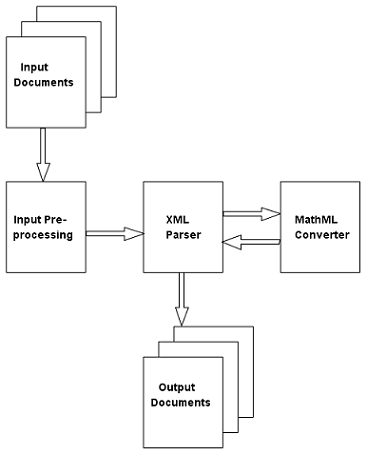
\includegraphics{basic_diagram}
\caption{Basic diagram of application workflow}
\label{fig:basicworkflow}
\end{figure}

This thesis is a~continuation of my Bachelor thesis~\cite{Kucbel2011thesis} called \textit{Generování textu z MathML}. The bachelor thesis introduces a~program for generating plain text from MathML as described in the paragraph above. However, it has serious limitations when it comes to scalability, supports only a~subset of the Presentation MathML elements, and a~limited amount of mathematical operations. The program uses XSL Transformations to convert MathML markup into the plain text format. In this thesis we will try to improve the computation speed, provide better scalability, support a~greater amount of mathematical operations, and encompass most of the Presentation MathML as well as the Content MathML elements.

Before input documents are loaded into an in-memory structure for representing XML documents, a~preprocessing phase will take place. This includes determining the file structure on the hard-drive, and retrieving all files from the input document and all its descendants. This structure will be preserved, and output documents will have the same structure~- just in the user-specified directory. Also, input files can be packed using the .zip archive file format (as is the case with documents in the MREC~\ref{section:mrec}), and such files have to be unpacked before further processing. Then, if requested, we will canonicalize input files. Since the canonicalization comes from external module (library), we have to be careful of possible errors or the time efficiency of this process. 

One important factor about the input documents that was not taken into account is their quantity. The application must be able to process large corpora of mathematical documents in reasonable time and with efficient memory usage. Fortunately, modern computation systems provide a~way of running the application in multiple threads. The application just has to ensure that all threads work with the same settings. This can be accomplished by providing a~single point of entry to the settings instance. A~globally visible class (object) that implements the Singleton design pattern is the best solution for accessing settings across the whole application. Also, retrieving external resources for each single thread is very time consuming. Therefore, an in-memory cache of resources common for all threads will be implemented.

We can now create a~more complex and detailed diagram of internal workings and dataflows inside the application (see Figure~\ref{fig:activitydiagramall}). 

\begin{figure}[!ht]
\centering
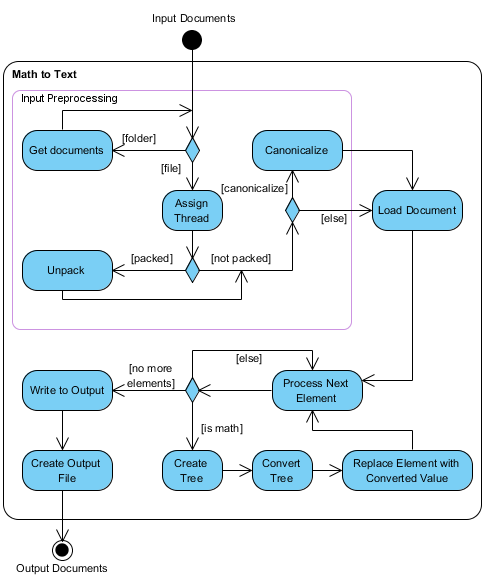
\includegraphics[width=\textwidth]{activity_diagram_all}
\caption{Activity diagram of the application}
\label{fig:activitydiagramall}
\end{figure}
\newpage
Three activities (processes) still remain to be defined:
\begin{enumerate}
\item Load Document,
\item Create Tree,
\item Convert Tree.
\end{enumerate}

\section{Load Document}
\label{section:loaddocument}
When it comes to processing XML documents, there are four common approaches:

\begin{enumerate}
\item Document Object Model\footnote{\url{http://www.w3.org/DOM/DOMTR}} (DOM) retains the tree structure of the XML document and is composed of nodes. Node represents elements in the XML structure and form a~hierarchical structure.

\item Extensible Stylesheet Language\footnote{\url{http://www.w3.org/Style/XSL/}} (XSL) refers to a~family of languages used to transform and render XML documents. 

\item Streaming XML is an event-based, sequential, and unidirectional approach of processing XML documents.

\item XML data binding is a~process of mapping XML documents to objects in computer memory (deserialization).
\end{enumerate}

\begin{table}[!ht]
\centering
\begin{tabular}{|l|c|c|}
\hline
& Processing speed & Memory requirements \\ \hline
\hline
DOM & slow & high  \\ \hline
XSL & slow & high  \\ \hline
Streaming XML & fast & low  \\ \hline
Data binding & average & high  \\ \hline
\end{tabular}
\caption{XML processing options comparison}
\label{table:xmlprocessing}
\end{table}

The memory requirements shown in Table~\ref{table:xmlprocessing} stem from the maximum amount of data that each method uses to process documents. For Streaming XML method, which reads only one event at a~time and retains only minimal processing information, these requirements are low. The rest of compared methods need to load the whole document into computer memory, hence their memory requirements are high. The comparison of processing speeds comes from the experience of the author with using these methods.

Based on the comparison in Table~\ref{table:xmlprocessing} we choose the fastest and most memory-efficient method for processing our input documents~- the Streaming XML method. Algorithm~\ref{alg-processinput} shows a~way to process input documents using an in-memory tree structure defined in Section~\ref{section:createtree}.

\iffalse
\subsection{Document Object Model}
Document Object Model\footnote{Document Object Model \url{http://www.w3.org/DOM/DOMTR}} (DOM) is one of the most wide-spread methods of representing and working with XML and (X)HTML documents. It retains the tree structure of the XML document and is composed of nodes. Node represent elements in the XML structure and form a~hierarchical structure. 

Each node, except the top one called root, has a~parent. Nodes can have arbitrary amount of children or siblings (nodes with the same parent). This makes traversing the document structure very easy and logical. 

A major drawback of using DOM lies in creating the node tree for the whole document. The input document may be very extensive, but contains only a~few MathML expressions (pieces of MathML markup). We are only interested in these pieces and therefore a~lot of information provided by DOM is redundant and will be discarded. Also the memory and time requirements needed for creating DOM in computing memory increase with the size of input documents.

\subsection{XSL}
\label{section:xsl}
Extensible Stylesheet Language (XSL) is a~family of languages used to transform and render XML documents. It was created by the W3C consortium and consists of three languages:
\begin{itemize}
\item XSL Transformation,
\item XSL Formatting Objects,
\item XML Path Language.
\end{itemize}

\paragraph*{XSL Transformation (XSLT)} 
XSLT is a~language designed for transformation of XML documents into other XML documents, but can also be used to create different output formats, such as HTML, plain text XSL Formatting Objects. During this process the input documents stays unchanged, rather a~new document is created. 

XSLT employs special stylesheets to transform document. XSLT stylesheets consist of a~set of templates. Each template defines a~rule that describes how to process a~node that matches the template selector (most commonly an XPath expression). 

The transformation process follows a~simple algorithm: load stylesheets and create \textit{source tree} from the input document; starting at the root node apply the best matching template; continue till there are nodes to process. This method of processing makes XSLT a~declarative language.

\paragraph*{XSL Formatting Objects (XSL-FO)}
\label{xsl:xsl-fo}
XSL-FO document describes what the resulting pages look like and where the various components go, but does not specify the layout. XSL-FO documents are often created by transforming ordinary XML documents using XSL Transformation. An application called FO processor then takes these documents and converts them into some readable form, most often a~PDF or PS file. Several FO processor can be employed to achieve different results.

\paragraph*{XML Path Language (XPath)}
\label{xsl:xpath}
XPath is a~query language capable of selecting nodes in an XML documents. It also comes with a~multitude of functions, such as string operations, date functions or operations with numbers. 

XPath expression consists of three components: 
\begin{itemize}
\item an axis~- navigation within the tree (parent, child, sibling, $\ldots$);
\item a~node test~- match the node name to a~pattern;
\item zero or more predicates~- restricting a~node set based on conditions.
\end{itemize}

A disadvantage of XSL Transformations is the high time complexity. However modern XSLT processor employ optimization techniques and different tree representations which makes the transformation process perform better than general-purpose DOM implementations.

\subsection{Streaming XML}
Streaming approach of processing XML documents is event-based and sequential. It follows that there is no tree representation of the document created in the memory. In fact the memory requirements of streaming processing are minimal and often considered negligible. The streaming parser, after reporting an event, usually discards almost all of the information. However it keeps some of the data, for example a~list of unclosed nodes in order to catch possible errors. 

There is more than a~dozen available events that can be reported by the parser, such as:
\begin{itemize}
\item document start and end,
\item element start and end,
\item element text content,
\item comments.  
\end{itemize}

The parsing is unidirectional, the parser makes only one run through the document. Therefore every event is reported just once and there is no possibility of traversing the document structure. Hence the streaming processing comes into play when a~single pass through the document is sufficient.

Based on the method of reporting events, streaming parsers can be divided into two groups:
\begin{itemize}
\item push principle,
\item pull principle.
\end{itemize}

\paragraph*{Push Principle} When utilizing the push method of streaming XML documents all events are pushed (reported) to the application as soon as they are encountered in the document. The application needs to implement event handlers that will react to individual events and process them accordingly.

The industry standard for parsing based on push model is Simple API for XML (SAX) and has many implementations in multiple programming languages.

\paragraph*{Pull Principle} Unlike push method, with pull method the application requests the next event when it is ready to process it. The structure of the code that uses pull method resembles structure of XML documents, making it more readable and understandable than applications that use push methods.

There are various APIs that use pull method, among them XML Pull Parser (XPP)\footnote{\url{http://www.extreme.indiana.edu/xgws/xsoap/xpp/mxp1/index.html}}  and Streaming API for XML (StAX).

\subsection{XML Data Binding} XML data binding refers to a~process of mapping XML documents to objects in computer memory (deserialization). Objects in the application represent the types defined in the XML document (e.g. by XML Schema) and can be generated by various tools from XML Schema, minimizing the required for creating such objects (classes). 

The process of mapping XML types onto application objects is called \textit{unmarshalling}. The reverse process, serialization of objects, is called \textit{marshalling}. 

The obvious advantage of this method lies in the fact, that on application level we work only with objects and don't have to concern ourselves with XML specific issues. It makes the resulting code easily readable and comprehensive.

Unfortunately the disadvantages of XML data binding are numerous. The time and spacial requirements for marshalling and unmarshalling grow substantially with the size of input document. Also the round-trip (unmarshalling the document and then marshalling it back) may not preserve the sibling order of elements, physical structure of documents (CDATA sections), comments and entity references or DTDs.

Since MathML consists of hundreds of elements and each one has to be mapped to a~class when using XML data binding method, writing the bindings by hand is out of a~question. There is however an XML Schema of MathML available that could be used to generate said bindings. Unfortunately attempts of code generation from this schema failed. Moreover if MathML markup was embedded inside another XML markup, such as XHTML, the bindings for MathML only would not be sufficient. 

\subsection{Proposed Solution}
\label{section:inputProcessingSolution}
As we can see every method comes with many advantages as well as disadvantages making it the right choice in various situations. We will try to select one method, or a~combination of two methods, best suited for our use case and requirements. 

From the developer's point of view, the best solution would be to use XML data binding. However the above outlined disadvantages make it impossible to actually implement this method.

The next best approach is using the DOM with its easy to traverse structure. But there remains the issue of memory and time requirements needed to create the model. Going by these requirements the streaming method wins as it is the fastest and most memory-efficient method.

The optimal solution would be to pass through the document using the streaming method. But streaming method does not provide any means to look ahead or behind on elements that might be needed to process the current element. On the other hand the DOM method is well suited for accessing arbitrary elements in the document tree. So combining these two methods should lead to a~satisfactory solution. 

\paragraph*{Solution}\label{inputprocessing:solution} The streaming processor traverses the document and every read event that is not a~part of the MathML markup automatically writes to the output. As we can see, also the output document is being created dynamically. When the processor encounters a~\texttt{math} node it creates a~in-memory DOM-like representation of MathML tree. We use a~customized DOM-like model, because we do not actually need all the information that full DOM implementations tend to provide (such as namespaces), a~simpler implementation suffices. After the MathML model is created (\texttt{math} end element event gets registered) the conversion needs to take place immediately, so that the conversion result can be written to the output in the right place. This way all non-MathML related information is retained and written to the output and for every occurrence of MathML markup in the document a~separate DOM-like representation is created and directly converted. See Algorithm \ref{alg-processinput} for illustration. 
\fi

\begin{algorithm}[!ht]
\caption{Process input algorithm}
\label{alg-processinput}
\begin{algorithmic}[1]
\Procedure{ProcessInput}{}
	\State clear \texttt{tree}
	\Comment{a DOM-like MathML tree} 
	\While{next event exists}
		\State \texttt{event} $\gets$ next event
		\If{\texttt{event} is a~start of \texttt{math} element}
			\State \texttt{tree} $\gets$ create a~new tree
		\ElsIf{\texttt{event} is an end of \texttt{math} element}
			\State convert \texttt{tree} and write the result to the output
			\State clear \texttt{tree}			
		\ElsIf{\texttt{event} is inside \texttt{math} element}	
			\State insert a~new node, value or attribute in the \texttt{tree}
		\Else
			\State write \texttt{event} to the output
		\EndIf
	\EndWhile
\EndProcedure
\end{algorithmic}
\end{algorithm}

\section{Create Tree}
\label{section:createtree}
The tree in this case means an in-memory representation of MathML with a~tree structure. DOM seems like a~good option for this application; however, a~fully-fledged DOM representation of the MathML markup is not required. The information this model provides takes up a~lot of resources (time and memory) and a~big part of it would be discarded. However, we need a~structure that will provide a~comfortable traversal~- moving from parent to children and vice versa.

We have designed a~simplified DOM tree~- with just the information we actually need. Since we only use it to build a~tree representation of MathML markup, every node in this tree has a~special property that denotes its type~- name of the element and part of MathML it belongs to (Presentation or Content). 

Besides the type property, our simplified model contains a~list of children, pointer to the parent, a~text value, a~list of XML attributes (key-value pairs), and a~attribute that signifies whether this node has already been processed (we want to process each node only once).

Our very simple tree has one more advantage besides simplicity~- it allows the application to provide an option to change the method of loading XML documents.

\section{Convert Tree}
We are starting the conversion process with our tree representation of the MathML markup. At the beginning of the conversion, we need to determine whether the tree consist of only the Presentation markup, Content markup, or both, since each requires a~slightly different approach to the conversion. In most cases, the Presentation MathML resides directly in the \texttt{math} tree (is a~direct descendant of the \texttt{math} element) or in the element \texttt{semantics}, while the Content MathML is often found enclosed in the \texttt{annotation-xml} element with an attribute \texttt{encoding} set to the value \texttt{MathML-Content}. Or, we can simply traverse the tree till we find an element from either the Presentation or Content MathML markup and continue based on our finding.

The conversion process starts at the top level element, \texttt{math}, and then recursively continues to traverse the tree  converting the Presentation and Content elements based on their own specifics. Each converted node is marked as processed in order not to be processed twice. Since in some cases the conversion requires to look ahead and jump out of the recursion pattern to process a~sibling node (or any other node).

The basic outline of the conversion process can be seen in Figure~\ref{fig:converttree} and will be described in detail in the next sections.

\begin{figure}[!ht]
\centering
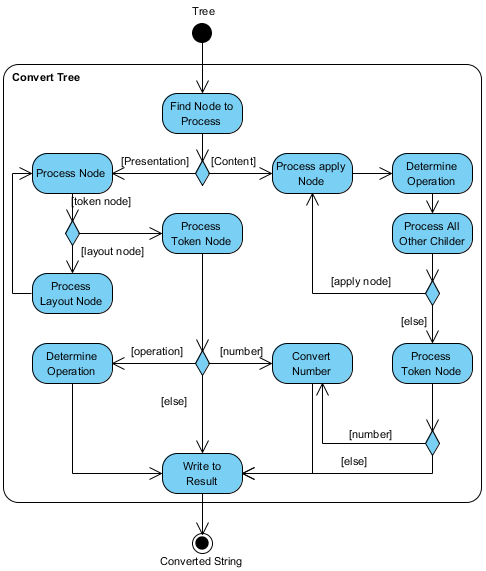
\includegraphics[width=\textwidth]{activity_diagram_tree}
\caption{Tree conversion process}
\label{fig:converttree}
\end{figure}

\subsection{Presentation MathML}
Every element of the Presentation MathML requires an individual approach to the processing. But there are still groups of elements with similar characteristics. 

The first group consists of token elements. The conversion is straightforward and depends only on the value of the element:
\begin{itemize}
\item \texttt{mn}~- convert number to string or take the original value,
\item \texttt{mi}~- take the original value if it is in Latin script, otherwise convert the value if possible (e.g. Greek alphabet),
\item \texttt{mo}~- determine the operation defined by the \texttt{mo} element value ($\Sigma \rightarrow$ sum, $\int \rightarrow$ integral, $\ldots$).
\end{itemize}
It is important to remember that one mathematical operation can be expressed with various symbols, and the conversion has to unify them into the same string representation.

The second group contains elements with a~specific purpose. In other words, these elements clearly state (with their names) what is their intended function. The conversion uses this fact and is therefore very simple. For example:
\begin{itemize}
\item \texttt{mfrac}~- fractions or binomial numbers,
\item \texttt{msqrt}~- square root,
\item \texttt{mfenced}~- subexpression is enclosed in parenthesis.
\end{itemize}

The third group is composed of elements that specify only the layout of the subexpression. To determine the exact function the author wanted to convey, we need additional information provided by child elements, and in some cases it may also depend on sibling or parent elements. 
\begin{figure}[!ht]
\lstset{language=XML,frame=lines}
\begin{lstlisting}
<math>
	<munder>
		<mo>lim</mo>
		<mrow>
			<mi>x</mi>
			<mo>&rarr;</mo>
			<mn>0</mn>
		</mrow>		
	</munder>
	<mrow>
		<msqrt>
			<mi>x</mi>
		</msqrt>
	</mrow>
</math>
\end{lstlisting}
\caption{Expression $\lim_{x \to 0}\sqrt{x}$ in Presentation MathML}
\label{fig:mathmllimit}
\end{figure}

As we can see in Figure~\ref{fig:mathmllimit}, the \texttt{munder} element has to be interpreted in the context of its child elements (especially the first child) and its first sibling element. Similar rules apply to elements \texttt{mover}, \texttt{munderover}, \texttt{msub}, \texttt{msup}, and \texttt{msubsup} that describe various mathematical constructs, such as summations, integrals, products, logarithms, and many more.

The last group is formed by elements that have a~purely presentation function: spacing, padding, and so on. These can be ignored altogether, since they do not provide any information about the meaning of presented expressions.


\subsection{Content MathML}
\label{section:analysis-content}
The cornerstone of the Content MathML is without a~doubt the element \texttt{apply}~- the function application. It describes the application of its first child element on the rest of child elements~- all of which can be \texttt{apply} elements themselves. The \texttt{apply} element will, therefore, serve as a~hub~- assigning the processing of expression or subexpression based on the operator (the first child element).

To be able to convert the expression correctly, we need a~different approach than for the Presentation MathML, where the elements are ordered for display purposes and can be converted basically from top to bottom (with a~few exceptions). In the Content MathML a~function can be applied to multiple elements, but it will be declared only once as seen in Figure~\ref{fig:mathplus} (in the Presentation MathML the plus symbol would be declared twice~- between $x$ and $y$, $y$ and $z$).

\begin{figure}[!ht]
\lstset{language=XML,frame=lines}
\begin{lstlisting}
<math>
	<apply>
		<plus/>
		<ci>x</ci>
		<ci>y</ci>
		<ci>z</ci>
	</apply>
</math>
\end{lstlisting}
\caption{Expression $x+y+z$ in Content MathML}
\label{fig:mathplus}
\end{figure}

Therefore, we can not determine word order of the expression from the position of elements in the document (as is the case in the Presentation MathML), but we have to specify the desired word order for each operation separately. Fortunately, operations can be sorted into logical groups based on the word order we use when presenting them.

\begin{itemize}
\item Infix form~- the operator is used between pairs of inputs~- starting with the first and the second input, then the second and the third and so on. These include operators for division ($x/y/z$), multiplication ($x\cdot y\cdot z$), comparison ($x=y=z, \geq, <$), and many more.

\item  Prefix form~- the operator is used at the beginning; preceding inputs. In this case, the operator is used only once at the beginning followed by converted inputs. Examples include absolute value ($|x|$), negation ($\neg$), or floor ($\lfloor x \rfloor$).

\item Prefix form with multiple inputs~- a~special case of the prefix form, where there are multiple inputs. In this instance, the operator is also used only once, but inputs have to be divided by commas, and the last two inputs divided by the word "and". Function $min(x,y,z)$ should be converted to string: minimum of $x$, $y$ and $z$. Another examples might be sets, lists, functions greatest common divisor, maximum, or lowest common multiple.

\item Quotient and remainder~- $rem(x,y)$ should be converted to: reminder of $x$ divided by $y$. Similarly the quotient operator.

\item Others~- operators that do not belong to any of abovementioned categories or belong to more than one (like plus or minus, which can be used in both the prefix and infix form) have to be treated in a~separate way.
\end{itemize}

\subsection{Operators and Symbols}
As we mentioned before, many mathematical operations can be expressed using more than one operator or symbol. Our task lies in identifying operators and symbols belonging to each operation, creating a~storage structure for this data, and developing a~method or methods for searching in this structure, i.e., finding an operation for a~given operator. 

This way, all operators that denote the same operation are grouped together, and we can easily unify the way each operation is converted.

\subsection{Adding Parentheses}
Imagine someone read you the following sentence: "x to the power of three plus y". What equation would you imagine? Is it $x^{3} + y$? Or $x^{3+y}$? Lets assume the original equation was the latter, $x^{3+y}$. In the MathML markup this ambiguity does not exist~- as can be seen in Figure~\ref{fig:addingbraces}. However, the Presentation MathML relies on the rendering of the equation and the ability of the user to visually distinguish between the two possibilities (standard font vs superscript), and so does not need to explicitly include parentheses. The Content MathML is not predominantly intended to be read by human users, and, therefore, it does not provide explicit parentheses.

\begin{figure}[!ht]
\lstset{language=XML,frame=lines}
\begin{lstlisting}
<math>
	<mrow>
		<msup>
			<mi>x</mi>
			<mrow>
				<mn>3</mn>
				<mo>+</mo>
				<mi>y</mi>
			</mrow>
		</msup>
	</mrow>
	<annotation-xml encoding="MathML-Content">
		<apply>
			<power/>
			<ci>x</ci>
			<apply>
				<plus/>
				<cn>3</cn>
				<ci>y</ci>
			</apply>
		</apply>
	</annotation-xml>
</math>
\end{lstlisting}
\caption{Expression $x^{3+y}$ in Presentation and Content MathML}
\label{fig:addingbraces}
\end{figure}

Since the conversion results is just a~plain text with no visual aid to determine what the original equation was expressing, we have to enclose parts of equations that logically belong together and can be ambiguous with parentheses ourselves. 

In the Presentation MathML logical parts of equations reside inside a~single \texttt{mrow} element. So the straightforward solution is to prepend and append parentheses to the \texttt{mrow} element content. However, we do not always need (or want) parentheses in this place, like in the case of the \texttt{msup} element in Figure~\ref{fig:addingbraces}. The easiest, and in most cases sufficient fix, is to add parentheses only if the \texttt{mrow} element has at least two child elements.

In the Content MathML the element \texttt{apply} acts as a~grouping element. Similarly to the \texttt{mrow} element, we do not need to add parentheses every time. In Figure~\ref{fig:addingbraces} the first \texttt{apply} element does not need to use parentheses~- only the second one does. For deciding whether to add parentheses or not, we will use the division of operations introduced in Section~\ref{section:analysis-content}. Only operators belonging to the \textit{infix} form group will add parentheses.

The resulting string procured from the conversion of equation $x^{3+y}$ should be: "x to the power of open braces three plus y close braces".

\subsection{Localization}
Every string  that is outputted has to be localized to the user specified language. The exception are token elements that are copied verbatim. There is a~problem with different word order in different languages. We will, however, work with just Germanic and Slavic languages that have very similar word order (as opposed to Japanese, which puts verb at the end of the sentence). We can, therefore, work with a~simple word substitution for localization and don't have to occupy ourselves with diverse word orders.

\chapter{Implementation}
\label{chapter:implementation}
This chapter describes various implementation aspects that occurred during the creation of the conversion application. The application is written in the Java programming language~- mainly because of personal preference of the author. Also, the existence and availability of many frameworks and tools for Java language (for working with XML documents among others) are big advantages of using this language. 

The application uses Apache Maven for build automation, distribution management, and dependency management.

The structure of the application can be seen on the component diagram~\ref{fig:componentdiagram} below.

\begin{figure}[!ht]
\centering
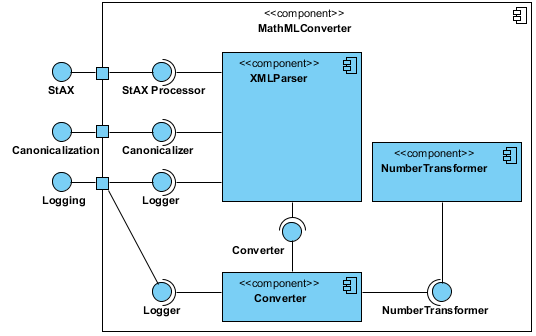
\includegraphics[width=\textwidth]{component_diagram}
\caption{Component diagram of the application}
\label{fig:componentdiagram}
\end{figure}

\section{DOM-like Representation of MathML}
The implementation of the tree designed in Section~\ref{section:createtree} can be seen in Figure~\ref{fig:customdom}.

\begin{figure}[!ht]
\lstset{language=Java,frame=single,backgroundcolor=\color{lightgray}}
\begin{lstlisting}
public final class MathMLNode {
    /**
     * Type of this node.
     */
    private MathMLElement type;
    /**
     * List of all children of this node. Empty if 
     * there are none. In this case value must be 
     * set.
     */
    private List<MathMLNode> children = new ArrayList<MathMLNode>();
    /**
     * Text value of this node. {@code null} if 
     * there are some child nodes.
     */
    private String value;
    /**
     * Parent node.
     */
    private MathMLNode parent;
    /**
     * Was this node already processed? Useful when 
     * you have to "look ahead" and process
     * element sooner.
     */
    private boolean processed = false;
    /**
     * Set of attributes.
     */
    private Set<XmlAttribute> attributes = new HashSet<XmlAttribute>();
    
    ... getters
    ... setters
\end{lstlisting}
\caption{Simplified DOM for internal representation of MathML markup}
\label{fig:customdom}
\end{figure}

\section{Input Processing}
As we outlined in Section~\ref{section:loaddocument}, the streaming approach with custom DOM-like internal representation of the MathML markup is used. 

In Java, two major APIs\footnote{Application programming interface} for streaming processing of XML documents are popular among developers:
\begin{itemize}
\item SAX (Simple API for XML) implements the push principle~- the reporting of events as they are encountered.
\item StAX (Streaming API for XML)~- the pull principle. The application requests events from the StAX processor. (StAX is a~specification defined by the JSR 173\footnote{\url{http://www.jcp.org/en/jsr/detail?id=173}}.)
\end{itemize}

This application uses default StAX implementation that is shipped with Java Standard Edition 6 runtime, but there are also other implementations available, such as Woodstox\footnote{\url{http://woodstox.codehaus.org}} or Aalto\footnote{\url{http://wiki.fasterxml.com/AaltoHome}}. There is a~possibility to request one of these two implementations to use instead of the default implementation.

StAX offers two ways of traversing documents: Cursor API and Iterator API. We use the first, Cursor API, because it should be faster and more memory-efficient\footnote{\url{http://docs.oracle.com/cd/E17802_01/webservices/webservices/docs/1.6/tutorial/doc/SJSXP3.html}}. Two main interfaces are available in the Cursor API (Figure~\ref{fig:staxcursorapi}): \texttt{XMLStremReader} for accessing all possible information retrievable from XML documents and \texttt{XMLStreamWriter} which in turn provides methods for outputting this information. 

\begin{figure}[!ht]
\lstset{language=Java,frame=single,backgroundcolor=\color{lightgray}}
\begin{lstlisting}
public interface XMLStreamReader {
	public int next();
   	public boolean hasNext();
   	public String getText();		
  	public String getLocalName();
  	public String getNamespaceURI();
  	...
} 

public interface XMLStreamWriter {
  	public void writeStartElement(String localName);
  	public void writeEndElement();
 	public void writeCharacters(String text);
	... 
}
\end{lstlisting}
\caption{Example of methods in \texttt{XMLStreamReader} and \texttt{XMLStreamWriter} interfaces of the Cursor API}
\label{fig:staxcursorapi}
\end{figure}

\subsection{XML Parser}
The implementation of the \texttt{XmlParser} interface~- \texttt{XmlParserStAX}~- is responsible for processing input XML documents using the StAX Cursor API, and at the same time creating output documents in the same run through the file. The internal processing follows steps outlined in the Algorithm~\ref{alg-processinput}. The parser also provides a~method for processing a~string input and producing a~string output. In this case, the parser processes the document defined by this string the same way as any other input document. However, the output contains only converted strings~- without any of original documents elements outside the MathML markup.
\begin{figure}[!ht]
\lstset{language=Java,frame=single,backgroundcolor=\color{lightgray}}
\begin{lstlisting}
public class XmlParserStAX implements XmlParser {
	public String parse(final String inputString, final Locale language);
	public File parse(final File file, final Locale language);
	public List<File> parse(final List<File> files, final Locale language);
}
\end{lstlisting}
\caption{Public methods of \texttt{XmlParserStAX} class}
\label{fig:xmlparserstax}
\end{figure}

The parser is capable of accepting a~folder as an input (instead of a~document) and processing all files in this folder, while preserving the file structure on the path entered by the user. 

A thread pool with a~user-specified size is initialized at the beginning of the conversion process, and for every file from the input a~\texttt{java.util.concurrent.Callable} instance is created. Using the \texttt{java.util.concurrent.ExecutorService} with our thread pool, these callables are concurrently invoked (whenever there is a~free thread in the thread pool, the next callable is invoked). 

A JDOM\footnote{\url{http://www.jdom.org}} implementation of the \texttt{XmlParser} is also provided and will be used to compare the performance of StAX implementation in Section~\ref{section:compareparsers}.

\section{Conversion}
When the parser creates a~complete tree, it immediately initializes the conversion of that tree by calling the \texttt{convert(tree, language)} method of the \texttt{MathMLConverter} class. The converter then decides which element of the input tree will be used as the root element of the conversion. The Presentation MathML markup has precedence over the Content markup, unless the opposite was requested by the user.

The converter consists of several classes that represent elements of MathML markup~- a~separate class for each element of the Presentation MathML markup and three classes (\texttt{Apply}, \texttt{Cn}, \texttt{Ci}) for the Content MathML markup. Every class has only one static method, \texttt{process(node, settings)} that is called whenever the traversal of the input tree encounters corresponding element. The run through the tree is done via the class \texttt{Node} and its static method \texttt{process(node, settings)}. This method works as a~switch for every type of node and delegates the processing to a~specific class. It also marks each encountered node as processed (see Figure~\ref{fig:converter-node} for illustration). The resulting string is gradually built from partial results of individual nodes.

\begin{figure}[!ht]
\lstset{language=Java,frame=single,backgroundcolor=\color{lightgray}}
\begin{lstlisting}
public class Node {
	public static String process(final MathMLNode node, final ConverterSettings settings) {
		final StringBuilder builder = new StringBuilder();
        switch (node.getType()) {
            ...
            case MN: {
                builder.append(Mn.process(node, settings));
                break;
            }
            case MFRAC: {    
                builder.append(Mfrac.process(node, settings));
                break;
            }
            ...
        }
        node.setProcessed();
    }    
}
\end{lstlisting}
\caption{Excerpt from the \texttt{Node} class}
\label{fig:converter-node}
\end{figure}

Before we get to the explanation of the conversion inside these classes, we have to define how mathematical operators and operations are defined in the application. The \texttt{Operation} class is an enumeration of all operations known to this application. Each operation is assigned a~unique key that is also used to retrieve appropriate textual representation of this operation from the localization files. Next, there is a~type of the operation as defined in Section~\ref{section:analysis-content}. The last property is an array of possible operators or symbols that might be used to represent this operation in documents. These can be standard HTML character entities entered by their name (\texttt{\&minus;}) or unicode code point (decimal or hexadecimal) or a~name of the corresponding element in the Content MathML markup as seen in Figure~\ref{fig:converter-operation}.

\begin{figure}[!ht]
\lstset{language=Java,frame=single,backgroundcolor=\color{lightgray}}
\begin{lstlisting}[mathescape=true]
public enum Operation {
	MINUS_PLUS("minus_plus", OperationType.INFIX,$~~$"&#8723;", "&#x2213;", "$\mp$");
}
\end{lstlisting}
\caption{An example of an operation}
\label{fig:converter-operation}
\end{figure}

The conversion of Presentation MathML elements is very simple and derives from the names of respective nodes. We offer special treatment for layout elements (such as \texttt{munder}, \texttt{msup}, $\ldots$) and distinguish a~few notable operations that occur often in mathematical texts~- limits, integrals, or summations. 

On the other hand, the conversion of Content MathML elements is more complicated. Everything important is happening inside the class \texttt{Apply}. The first child of the \texttt{apply} element denotes the operation. The operation can be defined by the appropriate Content MathML element, in which case we use the element name to retrieve the operation from the enumeration. It can also be defined by the \texttt{csymbol} element, then the value of the element is used, or by another \texttt{apply} element, for which we invoke the \texttt{Node.process()} method. 

When we have determined the exact operation, we proceed by processing it based on its type, i.e., based on its word order when spoken. Operations with a~type \texttt{OperationType.SPECIAL} have to be processed individually since they require a~distinctive approach (e.g., logarithm), or there are multiple ways of expressing them (e.g., summation, integral).

Lastly the conversion of numbers to strings ($11 \rightarrow$ eleven) is optionally executed, and contents of identifiers (elements \texttt{mi} and \texttt{ci}) are verbatim copied to the output. 

Example of results of the conversion can be found in Appendix~\ref{appendix:conversionexamples}.

\chapter{Results}
\label{chapter:results}
\section{Mathematical Retrieval Collection MREC}
\label{section:mrec}
MREC~\cite{mrec:mrec2011} is a~large corpus of mathematical texts (numbering close to 450~thousand documents). MREC\footnote{\url{https://mir.fi.muni.cz/MREC/index.html}} is based on documents downloaded from the arXMLiv\footnote{\url{http://kwarc.info/projects/arXMLiv/}}~\cite{mrec:arXMLiv2010}, which in turn is created by transforming \TeX~ documents from arXiv\footnote{\url{http://arxiv.org/}}~- a~huge library of freely available texts from multiple scientific fields including Physics, Mathematics, and Computer science. Using \LaTeX ML(described in the Subsection~\ref{section:latexml}), these texts are converted into the XML format with mathematics being represented in MathML. Not all documents from the arXiv are part of MREC~- only documents for which the conversion yielded results in categories successful and complete with errors are included.


\section{Comparing \texttt{XmlParser} Implementations}
\label{section:compareparsers}
The application comes with two implementations of the \texttt{XmlParser} interface: one uses DOM, the other StAX. Since the StAX implementation uses only general API, we have an option to use and compare different StAX API implementations. Together we have four implementations to test:
\begin{itemize}
\item JDOM~- a~DOM implementation,
\item Woodstox~- a~StAX implementation,
\item Aalto~- another StAX implementation,
\item StAX~- a~StAX implementation included in Java 6.
\end{itemize} 

The comparison will be performed on a~standard desktop computer with the following configuration: CPU Intel Core~i5-2400 (4 cores @3.1GHz), 8~GB RAM, standard HDD (7200~RPM) with Windows~8 64-bit and Java~7u21. Before we start comparing individual implementations, we will find the optimal number of threads to use. As we can see in Table~\ref{table:threadcount}, increasing the number of threads decreases computation time only until we use 10 threads, then the times stagnate or even slightly increase. Therefore, we will use 10 threads for comparison of \texttt{XmlParser} implementations.

\begin{table}[!ht]
\centering
\begin{tabular}{|c|c|}
\hline
Thread count & Time (s) \\ \hline
\hline
1 & 69.892 \\ \hline
2 & 38.295 \\ \hline
5 & 31.112 \\ \hline
10 & 21.414 \\ \hline
15 & 21.787 \\ \hline
25 & 22.114 \\ \hline
\end{tabular}
\caption{Running the application on 200 documents from MREC with variable thread count}
\label{table:threadcount}
\end{table}

Now we can start testing different implementations. For this purpose we will use a~sample of 2,000 MREC documents. We will focus not only on the computation time, but also on memory requirements represented by the heap size used by Java.

\begin{table}[!ht]
\centering
\begin{tabular}{|l|c|c|c|}
\hline
& Time (s) & Max. heap size (MB) & Max. used heap (MB) \\ \hline
\hline
StAX & 282.895 & 531.7 & 430.6 \\ \hline
Woodstox & 161.172 & 796.5 & 754.4 \\ \hline
Aalto & 167.264 & 797.5 & 740.5 \\ \hline
JDOM & 185.198 & 796.8 & 698.7 \\ \hline
\end{tabular}
\caption{A comparison of \texttt{XmlParser} implementations}
\label{table:comparison}
\end{table}

From Table~\ref{table:comparison} we can readily see that alternative StAX implementations are much faster than the implementation shipped with Java and also faster than JDOM. The memory usage of the three fastest implementations are roughly similar. However, from Table~\ref{table:averageheap} we can read that the average memory usage of JDOM is much higher than the rest of implementations. From this data we can deduce that Woodstox and Aalto implementations provide the best performance results. From this point forward we will use Woodstox implementation, because it has a~bigger user base, a~better documentation, and an active development.

\begin{table}[!ht]
\centering
\begin{tabular}{|l|c|c|c|}
\hline
& Average heap size (MB) \\ \hline
\hline
StAX & 350 \\ \hline
Woodstox & 500 \\ \hline
Aalto & 500 \\ \hline
JDOM & 700 \\ \hline
\end{tabular}
\caption{A comparison of \texttt{XmlParser} implementations' average heap sizes}
\label{table:averageheap}
\end{table}

\section{Converting the MREC Corpus}
The conversion was executed on a~fairly weak server. The same sample of 2,000 that was used in comparison of different \texttt{XmlParser} implementations took 37 seconds to complete. After a~preliminary testing, we found an optimal number of threads~- 10. The conversion process was run with the language option set to English, in 10 threads, and using the Woodstox StAX implementation.

\begin{table}[!ht]
\centering
\begin{tabular}{|c|c|}
\hline
Files converted & 439,423 \\ \hline
Time taken & 9,828,023 ms $\approx$ 164 min \\ \hline
Peak memory usage & 850 MB \\ \hline
Unrecognized operations & 4483 (unique) \\ \hline
Number of errors & 780 \\ \hline
\end{tabular}
\caption{Results of the conversion of the MREC corpus}
\label{table:mrecresults}
\end{table}

As we can see in Table~\ref{table:mrecresults} the conversion finished after 164 minutes and produced 780 errors. Most of these errors are caused by invalid or unexpected elements' position in the MathML structure. For example, the token element \texttt{mi}, which should contain only a~textual value, had a~child element. The \texttt{munder} element did not have two children.

The number of unique unrecognized operations is quite high. However, upon closer examination most of these operations are not defined by mathematical symbols (i.e., \texttt{swap}, \texttt{clique}, \texttt{prev}, $\ldots$). 

Overall the conversion was successful. Every input document was converted (judging by the number of resulting files). The number of unrecognized operations is reasonable (one unique operation per 98 files), the number of errors even lower (one error per 563 files).

\chapter{Conclusion}
At the beginning, the thesis examines MathML as a~format for storing and exchanging mathematical content. Tools for converting various formats into MathML and the need of a~single canonical representation of mathematical formulae in MathML are outlined and described. The thesis also introduces notable solutions that make mathematical content accessible for users with dyslexia or some form of visual impairment. 

With the acquired information the analysis of the problem is performed. During the analysis it became clear that the system developed as a~part of my Bachelor thesis is unsatisfactory in terms of MathML elements coverage and performance. A~completely new system is designed. Streaming XML is proposed as the best method of processing XML documents. Every occurrence of the MathML markup in the input document is loaded into a~custom simplified tree and thereafter converted into plain text format. 

The resulting implementation provides a~localization into three languages~- English, Slovak, and Czech. Also, many settings for the application are available, including a~possibility to swap StAX implementations.  

In the last chapter the results of running the application on a~substantial amount of documents from the MREC corpus are shown. 

For a~future work, a~framework for defining mathematical operations via external files could be implemented. This will pose a~few problems with the word order of user defined operations, especially in the Content MathML. Also, the application could be translated into more languages. 

\clearpage
\markboth{Bibliography}{Bibliography}
\bibliographystyle{own}
\bibliography{thesis}

\appendix
\chapter{Conversion Examples}
\label{appendix:conversionexamples}

\begin{figure}[!ht]
\lstset{language=XML,frame=lines}
\begin{lstlisting}
<?xml version="1.0" encoding="UTF-8"?><document xmlns:m="http://www.w3.org/1998/Math/MathML" xmlns:conv="http://code.google.com/p/mathml-converter/">
	<child id="42">
		<content>content</content>		
		<conv:math>logarithm to the base two of open braces x plus five point two close braces</conv:math>
		<content></content>
	</child>
	<conv:math>logarithm to the base two of open braces x plus five point two close braces</conv:math>
</document>
\end{lstlisting}
\caption{Figure~\ref{appendix:xml:example1} converted using StAX}
\end{figure}

\begin{figure}[!ht]
\lstset{language=XML,frame=lines}
\begin{lstlisting}
<?xml version="1.0" encoding="UTF-8"?>
<document xmlns:m="http://www.w3.org/1998/Math/MathML">
	<child id="42">
		<content>content</content>		
		<m:math>
			<m:mrow>
				<m:msub>
					<m:mo>log</m:mo>
					<m:mn>2</m:mn>
				</m:msub>
				<m:mrow>
					<m:mi>x</m:mi>
					<m:mo>+</m:mo>
					<m:mn>5.2</m:mn>
				</m:mrow>
			</m:mrow>			
		</m:math>
		<content/>
	</child>
	<m:math>
		<m:semantics>
			<m:annotation-xml encoding="MathML-Content">
				<m:apply>
					<m:csymbol>log</m:csymbol>
					<m:logbase><m:cn>2</m:cn></m:logbase>
					<m:apply>
						<m:plus/>
						<m:ci>x</m:ci>
						<m:cn>5.2</m:cn>
					</m:apply>
				</m:apply>
			</m:annotation-xml>
		</m:semantics>
	</m:math>
</document>
\end{lstlisting}
\caption{Expression $log_2 (x+5.2)$ in MathML}
\label{appendix:xml:example1}
\end{figure}

\begin{figure}[!ht]
\lstset{language=XML,frame=lines}
\begin{lstlisting}
<?xml version="1.0" encoding="UTF-8"?><math xmlns="http://code.google.com/p/mathml-converter/">open braces sum from open braces i equals zero close braces to ten of open braces absolute value of i factorial minus x with lower index i end absolute value close braces close braces times definite integral from 0 to 1 of x with respect to x</math>
\end{lstlisting}
\caption{Figure~\ref{appendix:xml:example2} converted using StAX}
\end{figure}

\begin{figure}[!ht]
\lstset{language=XML,frame=lines}
\begin{lstlisting}
<math xmlns="http://www.w3.org/1998/Math/MathML">
	<mrow>
		<mrow>
			<munderover>
				<mo>&#x2211;</mo>
				<mrow>
					<mi>i</mi>
					<mo>=</mo>
					<mn>0</mn>
				</mrow>
				<mn>10</mn>
			</munderover>
			<mrow>
				<mo>|</mo>
				<mi>i</mi>
				<mo>!</mo>
				<mo>-</mo>
				<msub>
					<mi>x</mi>
					<mi>i</mi>
				</msub>
				<mo>|</mo>
			</mrow>
		</mrow>
		<mo>*</mo>
		<msubsup>
			<mi>&#x222b;</mi>
			<mi>0</mi>
			<mi>1</mi>
		</msubsup>
		<mi>x</mi>
		<mo>&#x2146;</mo>
		<mi>x</mi>
	</mrow>
</math>
\end{lstlisting}
\caption{Expression $\Sigma_{i=10}^{10}|i!-x_i|*\int_0^1 x \mathrm{d} x$ in MathML}
\label{appendix:xml:example2}
\end{figure}

\end{document}